% !TEX encoding   = UTF8
% !TEX spellcheck = ru_RU
% !TEX root = ../seminars.tex

%%=============================
\chapter{Потоки ввода и вывода}
%%=============================

%%==========================
\section{Записи температуры}
%%==========================
Рассмотрим упражнение~2 из~\textbookref{главы~10}. Идею записи температуры выразим согласно тексту \textbookref{раздела~10.5} учебника:

\cppfile[firstline=9, lastline=13]{projects/09/store_temps.cpp}



%%========================
\paragraph{Запись в файл.}
%%========================
Легко написать функцию, которая сохранит готовые записи в~простом формате.

\cppfile[firstline=42, lastline=50]{projects/09/store_temps.cpp}

\noindent Тогда функция \code{main} может принять такой вид:

\cppfile[firstline=52, lastline=52]{projects/09/store_temps.cpp}
\cppfile[firstline=54, lastline=57]{projects/09/store_temps.cpp}



%%==========================
\paragraph{Тестовые данные.}
%%==========================
Попробуем генерировать температурные записи случайным образом. Для~правдоподобия зададим синусоидальное поведение в~течение дня. Примерно к~2 часам дня наблюдается максимум нагрева, а ночью земля остывает, и достигается минимум. Конечно, мы не~принимаем в~расчёт движение воздушных масс, облачность и прочее.

\begin{center}
  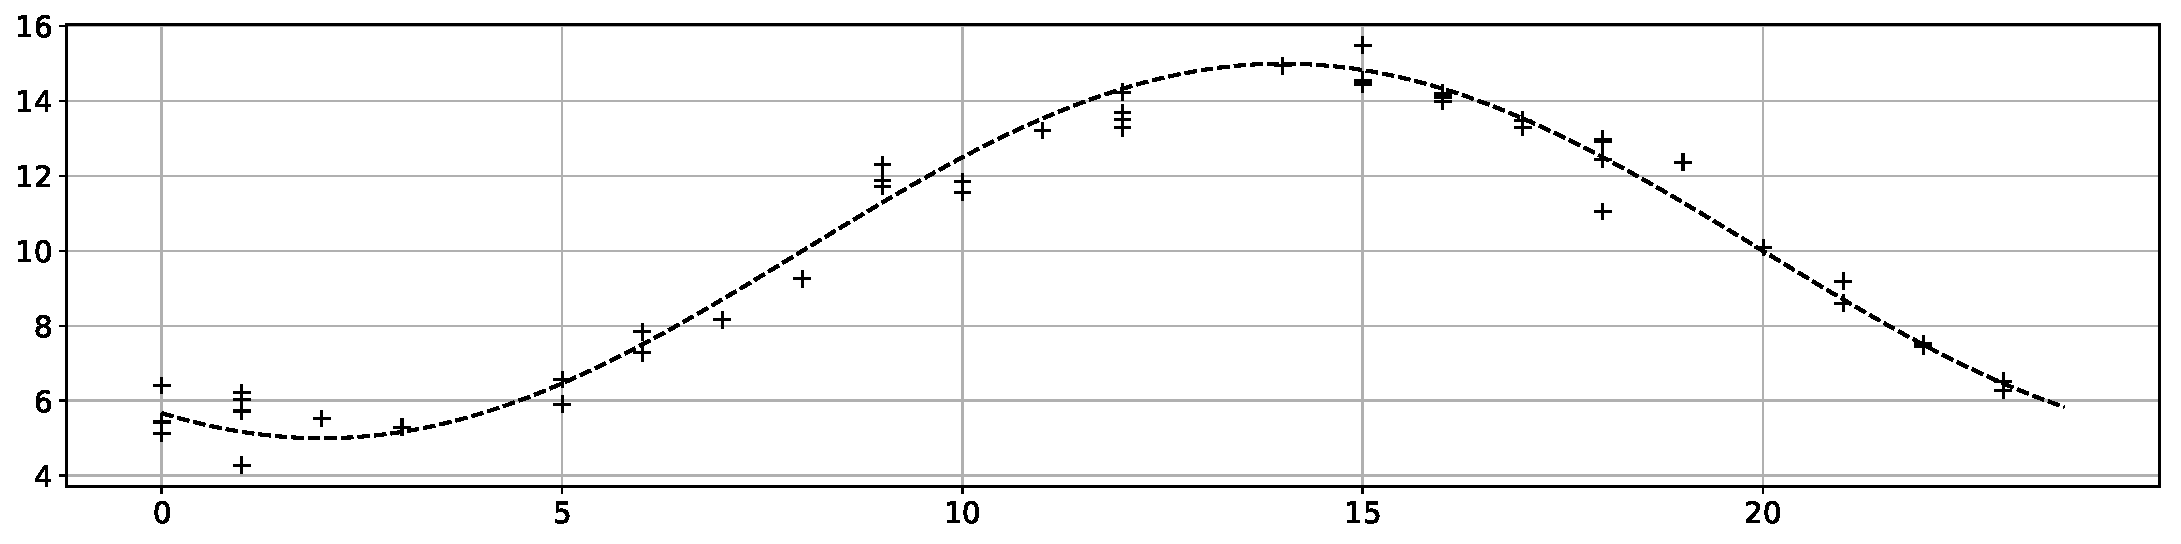
\includegraphics[width=0.8\textwidth]{images/raw_temps.pdf}
\end{center}

\cppfile[firstline=21, lastline=40]{projects/09/store_temps.cpp}

При~генерации записи мы случайным образом выбираем время суток, когда измерение произведено. А затем используем синусоиду с~некоторыми фиксированными параметрами: среднее в~течение дня, амплитуда колебаний за~день "--- для~вычисления текущего среднего значения и добавляем случайное отклонение по~нормальному закону распределения.



%%================================
\paragraph{Псевдослучайные числа.}
%%================================
Напомним, что функция плотности вероятности нормального распределения задаётся следующим соотношением:
\[
  p(x|\mu, \sigma) = \frac{1}{\sigma\sqrt{2\pi}} \cdot
                     \exp\left( -\frac{(x - \mu)^2}{2\sigma^2} \right)
\]
\noindent где \(\mu\) "--- среднее значение случайной величины \(x\), а \(\sigma\) "--- её стандартное отклонение. Величина \(\sigma\) означает, что с~вероятностью \(\approx 68\%\) значения \(x\) будут в~диапазоне \([\mu - \sigma, \mu + \sigma]\).

Рассмотрим определение функции, генерирующей псевдослучайное целое число в~заданном диапазоне из~заголовочного файла \code{std\_lib\_facilities.h}.

\cppfile[firstline=247, lastline=253]{projects/lib/std_lib_facilities.h}

По~аналогии, руководствуясь стандартом языка в~качестве справочника, пишем функцию генерирующую псевдослучайное число с~нормальным распределением.

\cppfile[firstline=15, lastline=19]{projects/09/store_temps.cpp}

\noindent Если необходимо генерировать различные последовательности псевдослучайных чисел при~разных запусках, следует задать произвольное начальное значение (\textenglish{seed}) генератору.

\begin{cppcode*}{linenos=false}
  static default_random_engine ran{time(nullptr)};
\end{cppcode*}



%%==========================
\paragraph{Чтение из файла.}
%%==========================
Продолжим работу с~записями и перейдём к~упражнению~3. Добавим оператор чтения из~потока ввода.

\cppfile[firstline=14, lastline=21]{projects/09/temp_stats.cpp}

\noindent
Заметьте, мы упустили из~вида проверку корректности входных данных! Добавьте её самостоятельно. После этого, записи можно прочитать из~файла следующим образом:

\cppfile[firstline=23, lastline=39]{projects/09/temp_stats.cpp}

\noindent
и организовать функцию \code{main} так:

\cppfile[firstline=65, lastline=65]{projects/09/temp_stats.cpp}
\cppfile[firstline=67, lastline=73]{projects/09/temp_stats.cpp}



%%==================
\section{Сортировка}
%%==================
Для~вычисления медианы нам понадобится упорядочить записи по~температуре. Выполним это, используя лямбда-выражение в~качестве критерия сортировки.

\cppfile[firstline=52, lastline=54]{projects/09/temp_stats.cpp}

Поскольку входные данные функции желательно не~изменять, а сортировка меняет порядок, нам понадобится копия вектора записей температур в~функции \code{temp\_stats}. Для~удобства инициализации этой копии, передадим её по~значению (!):

\cppfile[firstline=41, lastline=42]{projects/09/temp_stats.cpp}
\cpp`  // ...`
\cppfile[firstline=62, lastline=63]{projects/09/temp_stats.cpp}



%%========================
\section{Лямбда-выражения}\label{sect:lambda}
%%========================
Лямбда-выражения появились в~стандарте \lang{C++11} и немного доработаны в~более позднем \lang{C++14}. По своей сути, это автоматически генерируемые компилятором аналоги \emph{функторов} "--- объектов классов, которые имитируют поведение функций.

Теперь вы уже способны создать аналог нашего лямбда-выражения в~\lang{C++03} самостоятельно:

\begin{cppcode*}{linenos=false}
struct ReadingLess
{
  bool operator() (const Reading& a, const Reading& b) const
  {
    return a.temperature < b.temperature;
  }
};
\end{cppcode*}

Благодаря перегрузке оператора \code{()} имитируется поведение функции, то есть объект можно вызвать синтаксически точно так же, как обычную функцию. Отсюда и происходит название "--- функтор. Тело метода, определённого внутри класса, является подставляемым (\code{inline}), что обеспечивает эффективность для~коротких функций.

\begin{cppcode*}{linenos=false}
Reading a, b;
...
ReadingLess compare;
if (compare (a, b))  // behaves as an ordinary function here
  ...
\end{cppcode*}

\noindent
Вызов алгоритма сортировки в~стиле \lang{C++03}:

\cpp/sort (temps.begin(), temps.end(), ReadingLess());/

Очевидно, объект класса способен на~большее, чем просто функция. Он может хранить некоторое состояние и с~его помощью менять поведение функции-метода. А также инициализировать это состояние при~помощи конструкторов и обеспечить доступ к~нему через вспомогательные методы.

Часть лямбда-выражения с~квадратными скобками \code{[]} "--- это инициализирующий захват (\textenglish{capture}), реализация которого обеспечивается конструктором класса. Через него можно передавать копию (или ссылку) окружения лямбда-выражения. Подробнее эта тема раскрывается в~книге \cite{Stroustrup:2013:en}.

Лямбда-выражения коротко и ясно выражают идеи, определяются по~месту использования, широко применяются в~качестве аргументов для~алгоритмов библиотеки STL (\textenglish{Standard Template Library}) и могут быть размещены в~контейнерах. При~этом часть работы, а именно, определение класса, выполняет компилятор вместо нас. Именовать лямбда-выражение необязательно.



%%================
\WhatToReadSection
%%================
\textcite{Stroustrup:2016:ru}: \textbf{глава~11}



%%===============
\ExercisesSection
%%===============
\begin{exercise}
    \item Разработайте текстовый формат файла для~хранения схемы логических элементов (см.~страницу~\pageref{par:logic:v1}).

    \item Выполните упражнения из~\textbookref{главы~10} учебника.
\end{exercise}
